\vspace{-0.09in}
\section{Model}
\label{sec:model}

Our non-parametric approach to solving one-shot learning is based on two components which we describe in the following subsections. First, our model architecture follows recent advances in neural networks augmented with memory (as discussed in Section~\ref{sec:relwork}). Given a (small) support set $S$, our model defines a function $c_S$ (or classifier) for each $S$, i.e. a mapping $S \rightarrow c_S(.)$. Second, we employ a training strategy which is tailored for one-shot learning from the support set $S$.

\vspace{-0.09in}
\subsection{Model Architecture}

\begin{figure}[t]
\centering
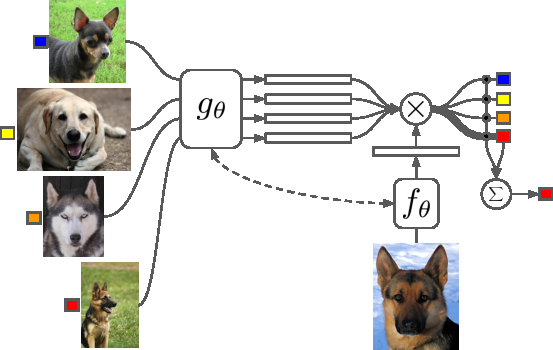
\includegraphics[width=.8\textwidth]{fig1}
\caption{\label{fig:arch}Matching Networks architecture}
\end{figure}

In recent years, many groups have investigated ways to augment neural network architectures with external memories and other components that make them more ``computer-like''. We draw inspiration from models such as sequence to sequence (seq2seq) with attention \cite{montreal}, memory networks \cite{memnets} and pointer networks \cite{ptrnets}.

In all these models, a neural attention mechanism, often fully differentiable, is defined to access (or read) a memory matrix which stores useful information to solve the task at hand. Typical uses of this include machine translation, speech recognition, or question answering. More generally, these architectures model $P(B|A)$ where $A$ and/or $B$ can be a sequence (like in seq2seq models), or, more interestingly for us, a set \cite{vinyals2015order}.

Our contribution is to cast the problem of one-shot learning within the set-to-set framework \cite{vinyals2015order}.
The key point is that when trained, Matching Networks are able to produce sensible test labels for unobserved classes \emph{without any changes to the network}.
More precisely, we wish to map from a (small) support set of $k$ examples of image-label pairs $S = \{(x_i, y_i)\}_{i=1}^k$ to a classifier $c_S(\hat{x})$ which, given a test example $\hat{x}$, defines a probability distribution over outputs $\hat{y}$.
We define the mapping $S\rightarrow c_S(\hat{x})$ to be $P(\hat{y} | \hat{x}, S)$ where $P$ is parameterised by a neural network. 
Thus, when given a new support set of examples $S'$ from which to one-shot learn, we simply use the parametric neural network defined by $P$ to make predictions about the appropriate label $\hat{y}$ for each test example $\hat{x}$: $P(\hat{y}|\hat{x}, S')$.
In general, our predicted output class for a given input unseen example $\hat{x}$ and a support set $S$ becomes $\arg\max_y P(y |\hat{x}, S)$.

Our model in its simplest form computes $\hat{y}$ as follows:

\begin{equation}
\hat{y} = \sum_{i=1}^{k} a(\hat{x},x_i) y_i
\label{eq:nn}
\end{equation}
where $x_i, y_i$ are the samples and labels from the support set $S=\{(x_i,y_i)\}_{i=1}^k$, and $a$ is an attention mechanism which we discuss below.
Note that eq.~\ref{eq:nn} essentially describes the output for a new class as a linear combination of the labels in the support set.
Where the attention mechanism $a$ is a kernel on $X\times X$, then \eqref{eq:nn} is akin to a kernel density estimator.
Where the attention mechanism is zero for the $b$ furthest $x_i$ from $\hat{x}$ according to some distance metric and an appropriate constant otherwise, then
\eqref{eq:nn} is equivalent to `$k-b$'-nearest neighbours (although this requires an extension to the attention mechanism that we describe in Section~\ref{sec:fce}).
Thus \eqref{eq:nn} subsumes both KDE and kNN methods.
Another view of \eqref{eq:nn} is where $a$ acts as an attention mechanism and the $y_i$ act as memories bound to the corresponding $x_i$.
In this case we can understand this as a particular kind of associative memory where, given an input, we ``point'' to the corresponding example in the support set, retrieving its label.
However, unlike other attentional memory mechanisms \cite{montreal}, \eqref{eq:nn} is non-parametric in nature: as the support set size grows, so does
the memory used.
Hence the functional form defined by the classifier $c_S(\hat{x})$ is very flexible and can adapt easily to any new support set.

\subsubsection{The Attention Kernel}
Equation~\ref{eq:nn} relies on choosing $a(.,.)$, the attention mechanism, which fully specifies the classifier. The simplest form that this takes (and which has very tight relationships with common attention models and kernel functions) is to use the softmax over the cosine distance $c$, i.e., 
$a(\hat{x},x_i) = e^{c(f(\hat{x}),g(x_i))} / \sum_{j=1}^k e^{c(f(\hat{x}),g(x_j))}$
with embedding functions $f$ and $g$ being appropriate neural networks (potentially with $f=g$) to embed $\hat{x}$ and $x_i$.
In our experiments we shall see examples where $f$ and $g$ are parameterised variously as deep convolutional networks for image tasks (as in VGG\cite{simonyan2014very} or Inception\cite{szegedy2015going}) or a simple form word embedding for language tasks (see Section~\ref{sec:results}).

We note that, though related to metric learning, the classifier defined by Equation~\ref{eq:nn} is discriminative. For a given support set $S$ and sample to classify $\hat{x}$, it is enough for $\hat{x}$ to be sufficiently aligned with pairs $(x',y') \in S$ such that $y'=y$ and misaligned with the rest. This kind of loss is also related to methods such as Neighborhood Component Analysis (NCA) \cite{nca}, triplet loss \cite{hoffer2015deep} or large margin nearest neighbor \cite{weinberger2009distance}.

However, the objective that we are trying to optimize is precisely aligned with multi-way, one-shot classification, and thus we expect it to perform better than its counterparts.
Additionally, the loss is simple and differentiable so that one can find the optimal parameters in an ``end-to-end'' fashion.

\subsubsection{Full Context Embeddings}
\label{sec:fce}
The main novelty of our model lies in reinterpreting a well studied framework (neural networks with external memories) to do one-shot learning. Closely related to metric learning, the embedding functions $f$ and $g$ act as a lift to feature space $X$ to achieve maximum accuracy through the classification function described in eq.~\ref{eq:nn}.

Despite the fact that the classification strategy is fully conditioned on the whole support set through $P(.|\hat{x},S)$, the embeddings on which we apply the cosine similarity to ``attend'', ``point'' or simply compute the nearest neighbor are myopic in the sense that each element $x_i$ gets embedded by $g(x_i)$ independently of other elements in the support set $S$. Furthermore, $S$ should be able to modify how we embed the test image $\hat{x}$ through $f$.

We propose embedding the elements of the set through a function which takes as input the full set $S$ in addition to $x_i$, i.e. $g$ becomes $g(x_i, S)$. Thus, as a function of the whole support set $S$, $g$ can modify how to embed $x_i$. This could be useful when some element $x_j$ is very close to $x_i$, in which case it may be beneficial to change the function with which we embed $x_i$ -- some evidence of this is discussed in Section~\ref{sec:results}.
We use a bidirectional Long-Short Term Memory (LSTM) \cite{hochreiter} to encode $x_i$ in the context of the support set $S$, considered as a sequence (see appendix for a more precise definition). 

The second issue can be fixed via an LSTM with read-attention over the whole set $S$, whose inputs are equal to $x$:
\begin{equation*}
f(\hat{x},S) = \text{attLSTM}(f'(\hat{x}), g(S), K)
\end{equation*}
where $f'(\hat{x})$ are the features (e.g., derived from a CNN) which are input to the LSTM (constant at each time step). $K$ is the fixed number of unrolling steps of the LSTM, and $g(S)$ is the set over which we attend, embedded with $g$. This allows for the model to potentially ignore some elements in the support set $S$, and adds ``depth'' to the computation of attention (see appendix for more details).

\subsection{Training Strategy}

In the previous subsection we described Matching Networks which map a support set to a classification function, $S \rightarrow c(\hat{x})$. We achieve this via a modification of the set-to-set paradigm augmented with attention, with the resulting mapping being of the form $P_\theta(.|\hat{x},S)$, noting that $\theta$ are the parameters of the model (i.e. of the embedding functions $f$ and $g$ described previously).

The training procedure has to be chosen carefully so as to match inference at test time. Our model has to perform well with support sets $S'$ which contain classes never seen during training.

More specifically, let us define a task $T$ as distribution over possible label sets $L$. Typically we consider $T$ to uniformly weight all data sets of up to a few unique classes (e.g., 5), with a few examples per class (e.g., up to 5).
In this case, a label set $L$ sampled from a task $T$,  $L \sim T$, will typically have 5 to 25 examples.

To form an ``episode'' to compute gradients and update our model, we first sample $L$ from $T$ (e.g., $L$ could be the label set $\{cats,dogs\}$). We then use $L$ to sample the support set $S$ and a batch $B$ (i.e., both $S$ and $B$ are labelled examples of cats and dogs).
The Matching Net is then trained to minimise the error predicting the labels in the batch $B$ conditioned on the support set $S$.
This is a form of meta-learning since the training procedure explicitly learns to learn from a given support set to minimise a loss over a batch.
More precisely, the Matching Nets training objective is as follows:
\begin{equation}
\theta = \arg\max_\theta E_{L \sim T} \left[ E_{S \sim L, B \sim L}\left[\sum_{(x,y) \in B} \log P_\theta\left(y|x, S\right)\right]\right].
\label{eqn:objf}
\end{equation}
Training $\theta$ with eq.~\ref{eqn:objf} yields a model which works well when sampling $S' \sim T'$ from a different distribution of novel labels. Crucially, our model does not need any fine tuning on the classes it has never seen due to its non-parametric nature. Obviously, as $T'$ diverges far from the $T$ from which we sampled to learn $\theta$, the model will not work -- we belabor this point further in Section~\ref{sec:imagenet}.